%; whizzy document
% latex beamer presentation.
% platex, latex-beamer でコンパイルすることを想定。 

%     Tokyo Debian Meeting resources
%     Copyright (C) 2007 Junichi Uekawa

%     This program is free software; you can redistribute it and/or modify
%     it under the terms of the GNU General Public License as published by
%     the Free Software Foundation; either version 2 of the License, or
%     (at your option) any later version.

%     This program is distributed in the hope that it will be useful,
%     but WITHOUT ANY WARRANTY; without even the implied warranty of
%     MERCHANTABILITY or FITNESS FOR A PARTICULAR PURPOSE.  See the
%     GNU General Public License for more details.

%     You should have received a copy of the GNU General Public License
%     along with this program; if not, write to the Free Software
%     Foundation, Inc., 51 Franklin St, Fifth Floor, Boston, MA  02110-1301 USA

% 実行順番
% sudo  ~/bin/usb-macbook-ir.c &
% real presentation (shell-command (concat "DISPLAY=:0.1 xpdf -fullscreen " (replace-regexp-in-string "tex$" "pdf"(buffer-file-name)) "&"))
% DISPLAY=:0.1 xpdf -fullscreen 

\documentclass[cjk,dvipdfmx,12pt]{beamer}
\usetheme{Tokyo}

%  preview (shell-command (concat "xpdf " (replace-regexp-in-string "tex$" "pdf"(buffer-file-name)) "&"))
%  presentation (shell-command (concat "xpdf -fullscreen " (replace-regexp-in-string "tex$" "pdf"(buffer-file-name)) "&"))

%http://www.naney.org/diki/dk/hyperref.html
%日本語EUC系環境の時
\AtBeginDvi{\special{pdf:tounicode EUC-UCS2}}
%シフトJIS系環境の時
%\AtBeginDvi{\special{pdf:tounicode 90ms-RKSJ-UCS2}}

\title{東京エリア Debian 勉強会}
\subtitle{資料}
\author{上川 純一 dancer@debian.org\\IRC nick: dancerj}
\date{2007年4月21日}
\logo{
\includegraphics[width=8cm]{image200607/openlogo-light.eps}}



% 三択問題用
\newcounter{santakucounter}
\newcommand{\santaku}[5]{%
\addtocounter{santakucounter}{1}
\frame{\frametitle{問題\arabic{santakucounter}. #1}
%問題\arabic{santakucounter}. #1
\begin{minipage}[t]{0.8\hsize}
 \begin{itemize}
 \item
      \begin{minipage}{0.2\hsize}
      
\includegraphics[width=0.9\hsize]{image200703/janken-A.png}\end{minipage} 
       \begin{minipage}{0.6\hsize}
       A #2\end{minipage}\\
 \item
      \begin{minipage}{0.2\hsize}
      
\includegraphics[width=0.9\hsize]{image200703/janken-B.png}\end{minipage} 
       \begin{minipage}{0.6\hsize}
       B #3\end{minipage}\\
 \item
      \begin{minipage}{0.2\hsize}
      
\includegraphics[width=0.9\hsize]{image200703/janken-C.png}\end{minipage} 
       \begin{minipage}{0.6\hsize}
       C #4\end{minipage}\\
 \end{itemize}
\end{minipage}
}
\frame{\frametitle{問題\arabic{santakucounter}. #1}
%問題\arabic{santakucounter}. #1
\begin{minipage}[t]{0.8\hsize}
\begin{itemize}
 \item
      \begin{minipage}{0.2\hsize}
      
\includegraphics[width=0.9\hsize]{image200703/janken-A.png}\end{minipage} 
       \begin{minipage}{0.6\hsize}
       A #2\end{minipage}\\
 \item
      \begin{minipage}{0.2\hsize}
      
\includegraphics[width=0.9\hsize]{image200703/janken-B.png}\end{minipage} 
       \begin{minipage}{0.6\hsize}
       B #3\end{minipage}\\
 \item
      \begin{minipage}{0.2\hsize}
      
\includegraphics[width=0.9\hsize]{image200703/janken-C.png}\end{minipage} 
       \begin{minipage}{0.6\hsize}
       C #4\end{minipage}\\
\end{itemize}
\end{minipage}
\begin{minipage}[t]{0.15\hsize}
答えは:

\vspace{1cm}

  {\huge \hspace{1cm}#5}
  \hspace{-6cm}\includegraphics[width=4cm]{image200703/janken-#5.png}
 \end{minipage}}
}

\begin{document}
\frame{\titlepage{}}

\section{Intro}

\begin{frame}
 \frametitle{本日のagenda}
\begin{minipage}[t]{0.4\hsize}
  \begin{itemize}
  \item 注意事項
	\begin{itemize}
	 \item 飲食禁止
	 \item 政治/宗教/営利活動禁止
	\end{itemize}
  \item 最近事情 etchのリリースについて
  \item 事前課題紹介
  \item quiz
 \end{itemize}
\end{minipage} 
\begin{minipage}[t]{0.4\hsize}
 \begin{itemize}
  \item quilt 
  \item darcs 
  \item git
 \end{itemize}
\end{minipage}
\end{frame}

\section{最近}

\begin{frame}
 \frametitle{OSCのagenda}
\begin{minipage}[t]{0.4\hsize}
  \begin{itemize}
   \item 仮想化友の会、Debian 勉強会の紹介
   \item 事前課題紹介
   \item 仮想化常識Quiz
 \end{itemize}
\end{minipage} 
\begin{minipage}[t]{0.4\hsize}
 \begin{itemize}
   \item Windowsから見える仮想化世界
   \item Debianの仮想化技術紹介
   \item 最後に
 \end{itemize}
\end{minipage}
\end{frame}

\begin{frame}
 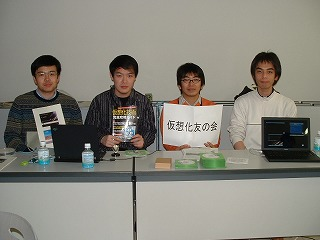
\includegraphics[width=0.5\hsize]{image200704/DSCF0063.jpg}
 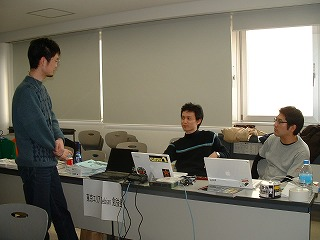
\includegraphics[width=0.5\hsize]{image200704/DSCF0064.jpg}
\end{frame}

\begin{frame}{etch リリース}
\begin{itemize}
 \item 4月8日 リリース
 \item 4月12日 宴会開催
 \item 4月XX日 日本語版リリースノート完成
\end{itemize}
\end{frame}

\begin{frame}

事前課題

「私はバージョン管理システムをこのようにつかっています」もしくは「バージョン管理システムを使わなくてすむようにこのようにしています」

\end{frame}

% (query-replace "\\subsection" "\\end{frame}\\begin{frame}")
\begin{frame}{青木さん}

VCSはCVSとSVNを使っていますが、あまり複雑なパッチ管理ではなく
単に共同開発の最新版管理レベルです。それとバックアップ的な意
味合いで使います。ハンドマージより凝ったことといえばVIMDIFの
利用ぐらいがせいぜいです。タグ管理はとくいではないです。DVCS
をつかうべきかと思いつつ、勉強不足ですね。

\end{frame}\begin{frame}{Kentaro Wakiさん}
\subsubsection{私はバージョン管理システムをこのようにつかっています}

特に変わった使いかたはしていません。
一応、プログラマなのでソースコードのバージョン管理に「subversion」使ってます。
つい最近まで「CVS」使ってました。
「subversion」で気に入ったのは、「ファイル名の変更」「ブランチの扱い」などです。また、「windows」ユーザと連係する場合に便利そうに見えます。
まだ実際には触ってませんが、「TortoiseSVN」は「windows」ユーザに違和感の少ないUIっぽいので。
「subversion」関連で、「Trac」の評判も良いようなので導入を検討しています。

\end{frame}\begin{frame}{森田尚さん}

\subsubsection{私はバージョン管理システムをこのようにつかっています}

個人で余暇に書いているプログラムのソースコード管理と、仕事(出版社で書籍
の企画・編集をしています)での原稿管理のために、Subversionリポジトリを
Apacheでホストして使っています。2002-2004年ごろは主にCVSを使っていました。

自分の仕事では、協働するチームメンバが複数の組織と拠点に分散していること
が多いので、いずれ分散型VCSを導入したいと考えています。

\subsubsection{バージョン管理システムを使わなくてすむようにこのようにしています}

数世代にわたるバックアップが欲しいだけのときなど、VCSを使うまでもない場
合のために、ホームディレクトリその他をpdumpfsのバックアップ対象にしてい
ます。

\end{frame}\begin{frame}{akeさん}

「バージョン管理システムを使わなくてすむようにこのようにしています」
何故バージョン管理システムが必要なのか?
一つの物に複数でよってたかって改変を加えるからである。
であれば、使わなくて済むようにするアプローチとして
\begin{itemize}
 \item 複数の改変を同時にしない
 \item 複数の改変が相互に影響しないようにする
\end{itemize}

のどちらかを行えば良いのである。
前者は改変を一人が行うと言う事になるが現実的ではない
後者を実現するためには、設計プロセスが完全でなければならない
要するに、ソフトウェア開発であれば、
モジュール化が適切に行われているなど、
設計の瑕疵を無くせばバージョン管理システムは不要である。
と言う事に行き着く。
\end{frame}\begin{frame}{akeさん}
実際の所、そう言った状況で作られるソフトウェアはまず無い。
多くの開発現場では、混沌の中から偶然の産物の様に作り出されたりする。
この状況が存在する限り、やはりバージョン管理システムは必要とされ続けるのだろう。
だが設計プロセスを注意深く行えば、設計プロセスの瑕疵を無くす手法が見つかれば、
なんとか実現できるかも知れない。

\end{frame}\begin{frame}{Hashimoto, Toruさん}

  今のソフトウェア開発プロジェクトでは、何とバージョン管理システムを使っ
ていない。複数の人が同じファイルを編集しようとすることも実際にあり、そ
の状況はかなり問題である。プロジェクト全体としてバージョン管理を導入す
る考えはないようである。そこで、自分のチーム内で独自にソースコードを管
理する方式を考えているところである。

  使用するツールとしてはSubversionを考えている。チームの担当範囲のファ
イルは決まっているので、バージョン管理対象は明確ではあるが、開発環境が
よく言えば特殊、悪く言えば洗練されていないために実際にきれいに適用する
のは一筋縄ではいかない。こんな環境でもうまく運用できる方法を考えている
ところである。

\end{frame}\begin{frame}{Hashimoto, Toruさん}
  その他、自分だけではあるがパッチ管理としてquiltを使ってみたことがあ
る。自分の変更点をパッチ(diff)にするのが自動的にできるのは便利だが、自
分の作業中に他人が同じファイルを編集するということが起こると混乱してし
まった。こういう用途には向かないようだ。

\end{frame}\begin{frame}{Noriaki Sato}

私はバージョン管理システムをこのようにつかっていたり、
いなかったりします(しました)

一年前まで:\\
バージョン管理システムを使ったことがありませんでした。
当時は、実験データ解析用のコードを書いていましたが、
\texttt{hoge\_{}20051204.cc} のようなファイル名だけで管理していました。
(頻繁に書き直したりするわけじゃないので、それで済んでいた)
CVS とか名前は知っていたけど、覚えている余裕がありませんでした。

\end{frame}\begin{frame}{Noriaki Sato}
一年前:\\
仕事で初めて VSS を使いました。
チェックアウトするとロックされてしまうのが不便じゃね?
と思いました。その後、VSS に上げる前のソースコードを
自分のローカルマシン上で管理するために Subversion を使っていました。
「達人プログラマ」で、ソースコード以外の普通のドキュメントも
バージョン管理システムで管理しよう、と言う話を読んで、
なるほど!と思いましたが、結局、今に至るまで実践はしていません。

\end{frame}\begin{frame}{Noriaki Sato}
今:\\
今度の現場では VSS を使わせてくれないらしいです。
それほどコードを書く必要のないプロジェクトなのですが、
台帳で管理するとか言う話です。
フリーソフトのインストールも不可なので、
svn を入れて使ったりする事も出来ません。
(一番つらいのは emacs(meadow) を使えない事なのですが、オフトピですね)


\end{frame}\begin{frame}{鈴木さん}
バージョン管理は、cvsとsubversionを使ったことがあります。
cvsは、Web(tlec.linux.or.jp)の更新で利用しています。チェックアウトすれば
どこでも更新
できるので便利です。最近余り更新してませんが。
subversionは、ドキュメント作成を会社と家で更新できるような1日の区切りで
チェックイン
していました。使ったり使わなかったりで持続しないです。理由は、リリースす
るときにtarに
まとめてバックアップしているので頻繁にsubversionは使ってないです。


\end{frame}\begin{frame}{H.Honjoさん}
個人で管理しているサーバに、バージョン管理システムとして
Subversionを、バグトラックシステムにはtracを利用しています。特に
変わった用途として使ってはおらず、通常どおりソースコード管理およ
びバグトラックとして使用しています。主にクライアントマシンとして
Windowsを使用している関係から、TortoiseSVNをSubversionのクライア
ントとして利用しています。

新たにリリースされたEtchへの移行を検討しており調査中ですが、
trac-ja-resourceパッケージがうまく動作してくれず、難航しています。

\end{frame}\begin{frame}{小室 文さん}
\subsubsection{バージョン管理システムを使わなくてすむようにこのようにしています}

バージョン管理は使っていません。会社ではバージョン管理を使うような人や案件はないです。
プライベートでも管理する物も一緒に管理したい人もいないので、導入していません。

バージョン管理を導入する場合、使う人が対等な位置にいるのが前提な気がします。なので、他の案件の一部分の機能を追加するためにファイルを検証サーバにアップする際は(1)事後報告するか(2)案件管理者にファイルを送る事が多いです。

使ってみないと!と思いつつも必要に迫られていないのでよく理解していません。


\end{frame}\begin{frame}{北原さん}

\subsubsection{バージョン管理システムを使わなくてすむようにこのようにしています}


回答:\\
個人的に作成しているプログラムはたいした量ではないので、「使わ
なくてすむように」というよりは、「使う必要がない」という状態です。  

プログラムを構成するファイルは、修正前にファイル名にバージョン番号を付け
て、全バージョンそのままの形で保存してあります。(若しくは、ディレクトリ
にバージョン番号を付けて丸ごとコピー。) 規模が小さいのでこれで十分管理
できてしまいます。

\end{frame}\begin{frame}{小林儀匡}

「私はバージョン管理システムをこのようにつかっています」

内容が日々進化していくファイル (プログラム・ドキュメント・翻訳・図など) 
は何でもリポジトリに入れてバージョン管理下に置いています。バージョン管
理システムのない生活はもう考えられなく、バージョン管理システムがあって
こそ効率的な仕事ができると思うようになっています。
\end{frame}\begin{frame}{小林儀匡}
これまでは主にSubversionなどの中央集権的なバージョン管理システムしか使っ
てきませんでしたが、最近、Debianのウェブサイトやリリースノートの日本語
訳コーディネータとして働くようになってから、分散バージョン管理システム
にも興味をもつようになりました。翻訳チーム全員にコミット権を与えるわけ
にはいかないというのはプロジェクトとしては仕方がないことだと思いますが、
他方でコーディネータとしては、あらゆるコントリビュータの仕事はきちんと
区別し、分割してコミットしたいのです。しかしそのような作業をコーディネー
タ一人でやるのは大変なので、分散バージョン管理システムを導入して、本家
リポジトリへのコミット権はもっていなくても自分のリポジトリにコミットで
きる翻訳者やレビューアにはどんどん自分で作業をしてもらったほうが、効率
がいいのではないかと思っています。

\end{frame}\begin{frame}{えとーさん}

\subsubsection{私はバージョン管理システムをこのようにつかっています}


自前のソースコードの管理や参加しているプロジェクトのソースコードの管理に
利用しています。

設定ファイルやその他雑多なものはあまり利用できていないので、今後も勉強しながら
便利に使っていきたいと思っています。


\end{frame}\begin{frame}{keng nakさん}

バージョン管理システムは、仕事で cvs をつかっています。ソー
スコードから word や excel の資料からメモに至るまですべて
まとめて cvs で管理していました。
今度配属されたプロジェクトでは Mercurial(OpenSolarisなど
で採用されている分散SCM)を使用することになり、今まで使っ
てきた cvs とは勝手が違うために戸惑っております。
今回は分散SCMが2種類紹介されるようですので、この機会に
分散SCMの有効な使い方を学べたらと思っています。
よろしくお願いします。


\end{frame}
\begin{frame}{でん@相模原さん}

従来、自作プログラムは環境情報をまとめたメモと一緒にソース
ファイル一式をtar.bz2で固めて蓄積してました。

この方法ではソースを管理すると言う点では問題は無いのですが
それ以外への発展が無く、方々の作業で無駄が発生しました。
代表的なのが、差分抽出により目的外の変更が入っていない事の
確認です。このような事をサポートしてくれるツールとして
バージョン管理ツールのDIFF機能を利用しています。
\end{frame}\begin{frame}{でん@相模原さん}
またバージョン管理業務を長く行っていると
\begin{itemize}
 \item   「何故バージョンを更新したのか」とか
 \item   「どうして、このような作りになっているのか」
\end{itemize}
といった事が忘れてしまいがちです。
このためバグトラッキングシステム(Trac)や自動ドキュメント化
システム(Doxygen)等との連携が今後の課題になっています。

今回のお題にはあがりませんでしたが、私は以下のようなシステム
で個人的には作業をしています。

\begin{itemize}
 \item バグトラッキング、仕様書管理
   → Trac
 \item バージョン管理
   → SubVersion/SVK
\end{itemize}

\end{frame}


\begin{frame}{Debian 常識クイズ}

Debian の常識、もちろん知ってますよね?
しらないとはずかしいけどしらないとは言えないいろいろなこと、
Debian Weekly News をベースに確認してみましょう。

\end{frame}

\santaku
{ウェブアプリケーション関連のパッケージの静的コンテンツはどこにおくべきか?}
{/var/www に置く}
{/usr/share/PACKAGE に置く}
{/srv/XXX に置く}
{B}


\santaku
{Debian Projectの MIA アカウントに対して 実施するWaTとは何をするもの
か}
{今年のDPL選挙に投票しなかった人に対して確認メールを送り反応がない人を引
退プロセスに移行する}
{気に入らない人を強制退会させる}
{あれ?Debian Developerだらけの水泳大会}
{A}


\santaku
{etch リリースはどういう暗号鍵で署名されるか?}
{オンライン鍵とオフライン鍵}
{オフライン鍵のみ}
{オンライン鍵のみ}
{A}

% オンライン鍵は、ネットワーク上にオンラインになっている鍵で、自動処理
%するためにパスフレーズすらない。


\santaku
{Frans PopがアナウンスしたBabelboxは何をするものか?}
{いろいろな言葉を喋ってくれる}
{フォントを複数表示}
{自動でくりかえし Debian Installer が稼働し、Gnomeにしばらくログインしてくれるしく
み}
{C}

\santaku
{DPL選挙の勝者は?}
{Iwamatsu}
{Sam Hocevar}
{Anthony Towns}
{B}


\begin{frame}{SCM特集}

 世界中に分散して開発しているオープンソース開発の現場では必須となるSCM。
 最近中央集権的なCVS・SVNから分散管理的なツールへの移行が進んでいます。
 最近の流行なんだけどあまりとりあげられていない現場のツール。その現状を
 特集してみます。

\begin{itemize}
 \item quilt
 \item darcs 
 \item git
\end{itemize}
\end{frame}

\begin{frame}[containsverbatim]{Debianのソース管理}

debian/changelog に変更履歴が記述されることになっている。
.dsc のバージョン毎の変更履歴は debdiff コマンドで確認できる。
ただし、各リリース単位でしか変更履歴の記録が存在しない。

\begin{verbatim}
$ ls -1  *dsc *.diff.gz *.orig.tar.gz
refit_0.7-1.diff.gz
refit_0.7-1.dsc
refit_0.7-2.diff.gz
refit_0.7-2.dsc
refit_0.7-3.diff.gz
refit_0.7-3.dsc
refit_0.7.orig.tar.gz
refit_0.8-1.diff.gz
refit_0.8-1.dsc
refit_0.8.orig.tar.gz
\end{verbatim}
\end{frame}

\begin{frame}[containsverbatim]{0.7-1, 0.7-2 の差分}

{\tiny

\begin{verbatim}

$ debdiff refit_0.7-{1,2}.dsc
diff -u refit-0.7/debian/README.Debian refit-0.7/debian/README.Debian
--- refit-0.7/debian/README.Debian
+++ refit-0.7/debian/README.Debian
@@ -6,4 +6,5 @@
-EFI files are available in /usr/share/refit/, bless refit.efi in a EFI
+EFI files are available in /usr/share/refit/, copy it to somewhere
+accessible from MacOSX, boot into Mac OS X, 'bless' refit.efi in a EFI
or HFSplus partition in order to use it.

- -- Junichi Uekawa <dancer@debian.org>, Sun,  2 Jul 2006 09:19:20 +0900
+ -- Junichi Uekawa <dancer@debian.org>, Sat,  8 Jul 2006 13:40:11 +0900
diff -u refit-0.7/debian/changelog refit-0.7/debian/changelog
--- refit-0.7/debian/changelog
+++ refit-0.7/debian/changelog
@@ -1,3 +1,10 @@
+refit (0.7-2) unstable; urgency=low
+
+  * README.Debian: update a little bit.
+  * remove gptsync.o from UNIX build so that it's not used in EFI build.
+
+ -- Junichi Uekawa <dancer@debian.org>  Sat,  8 Jul 2006 13:42:08 +0900
+
 refit (0.7-1) unstable; urgency=low

   * Initial release (Closes: #375999)
\end{verbatim}
} 
\end{frame}

\begin{frame}{SCMではないパッチの管理}
Debianのソースパッケージ内部にパッチファイルを複数保持し、変更単位に分離
して管理するシステム。パッチはパッケージの diff.gz に含まれる。

\begin{itemize}
 \item dpatch
 \item dbs
 \item quilt
\end{itemize}
 
\end{frame}

\begin{frame}

 quilt by 小林さん
\end{frame}


\begin{frame}

 darcs by David Smith
\end{frame}

\begin{frame}

 git-buildpackage by 上川
\end{frame}


\begin{frame}{git}

 git を日常的に使っている人

 挙手
\end{frame}

\begin{frame}{git}

 git の使いかたを知らない人

 挙手

\end{frame}

\begin{frame}{git}
 この会のメンバーは濃すぎるので、
 もう git の使い方は常識のようなので復習になってしまいますが

\end{frame}

\begin{frame}{git のワークフロー}
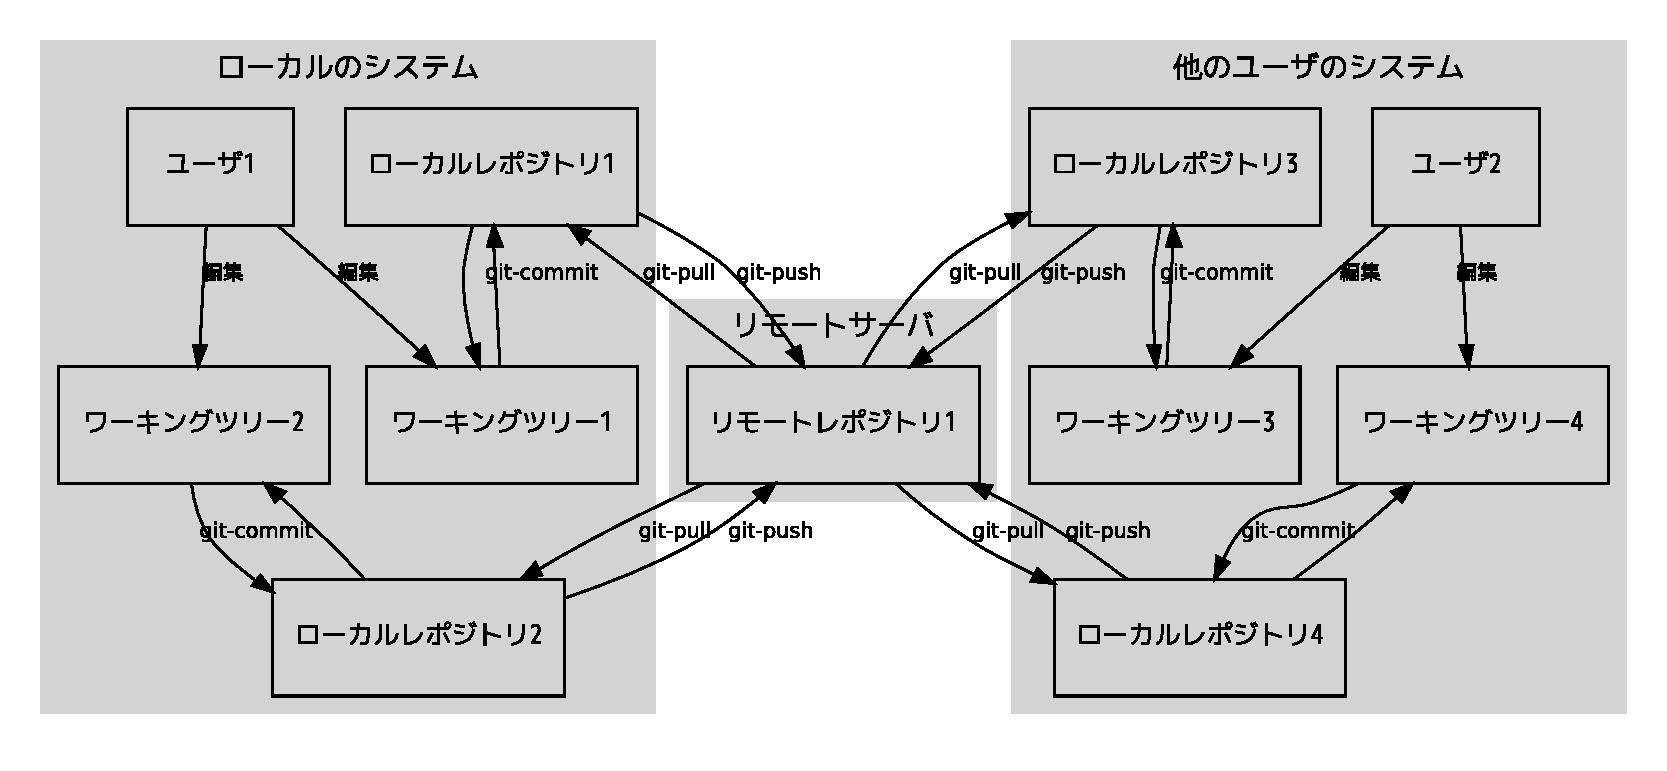
\includegraphics[width=1\hsize]{image200704/git-repos.eps}
\end{frame}

\begin{frame}{分散SCM、git の関連用語}

{\tiny
\begin{tabular}{|l|p{15em}|}
\hline
\hline
用語 & 定義 \\
\hline
 ワーキングツリー & SCMで管理されている作業用のディレクトリで、ユーザが
 直接作業できるようにファイルがある場所\\
\hline
 ローカルレポジトリ & SCMで管理されているデータ
 ワーキングツリーと同じ場所の
 .git ディレクトリに実体がある。直接ファイルを編集することはできない\\
\hline
 リモートレポジトリ & SCM管理されているデータで、
 ネットワーク上のどこかに存在し
 ているもの。しばしば他人と共有している。直接ファイルを編集することはで
 きない
\\
\hline
 コミット & ワーキングツリーからローカルレポジトリに情報を反映すること\\
\hline
 プッシュ & ローカルレポジトリからリモートレポジトリに情報を反映するこ
 と\\
\hline
 プル & リモートレポジトリからローカルレポジトリとワーキングツリーに情報を反映するこ
 と\\
\hline
\hline
\end{tabular}
}

\end{frame}


\begin{frame}{gitのよくつかうコマンド}

{\tiny 
\begin{tabular}{|l|l|p{15em}|l|}
\hline
\hline
コマンド名 &例 &意味 & cvs 相当\\
\hline
git-clone & git-clone {\it git://XXX/YYY} & 
 リモートレポジトリをローカルにクローンし、ワーキングツリーをチェックアウトする & cvs login, cvs co \\
\hline
git-init-db & git-init-db &
 ローカルレポジトリ(.gitディレクトリ)を作成する & cvs init\\
\hline
git-pull & git-pull {\it git://XXX/YYY} &
 リモートレポジトリの変更をローカルにマージし、ワーキングツリーを
 アップデートする & cvs up \\
\hline
git-commit & git-commit -a -m 'xxx' & 
 ローカルレポジトリに変更をコミットする & cvs ci の前半\\
\hline
git-push & git-push {\it git://XXX/YYY} & 
 ローカルレポジトリをリモートレポジトリに送信する & cvs ci の後半\\ 
\hline
git-add & git-add {\it filename}&
 ファイルを次回コミットの際にローカルレポジトリに追加されるように登録す
 る & cvs add \\
\hline
git-rm & git-rm {\it filename} & 
 ファイルを次回コミットの際にローカルレポジトリから削除されるように登録す
 る & cvs remove \\
\hline
git-status & git-status & 
 ローカルレポジトリに対してワーキングツリーの状況を確認する &
 cvs status\\
\hline
git-diff & git-diff & ローカルレポジトリとワーキングツリーの差分を
 表示する & cvs diff\\
\hline
\hline
\end{tabular}
}
\end{frame}

\begin{frame}{git-buildpackage 紹介}
 
Debian パッケージを管理する際のワークフローをスムーズにするためのツール
{\tiny 
\begin{itemize}
 \item arch-buildpackage - tools for maintaining Debian packages using arch
 \item cvs-buildpackage - A set of Debian package scripts for CVS source trees.
 \item darcs-buildpackage - Suite to help with Debian packages in Darcs archives
 \item git-buildpackage - Suite to help with Debian packages in Git repositories
 \item hg-buildpackage - Suite to help with Debian packages in Mercurial archives
 \item svn-buildpackage - helper programs to maintain Debian packages with Subversion
 \item tla-buildpackage - Suite to help with Debian packages in Arch archives
\end{itemize}
}
\end{frame}

\begin{frame}
 {git-buildpackage}
 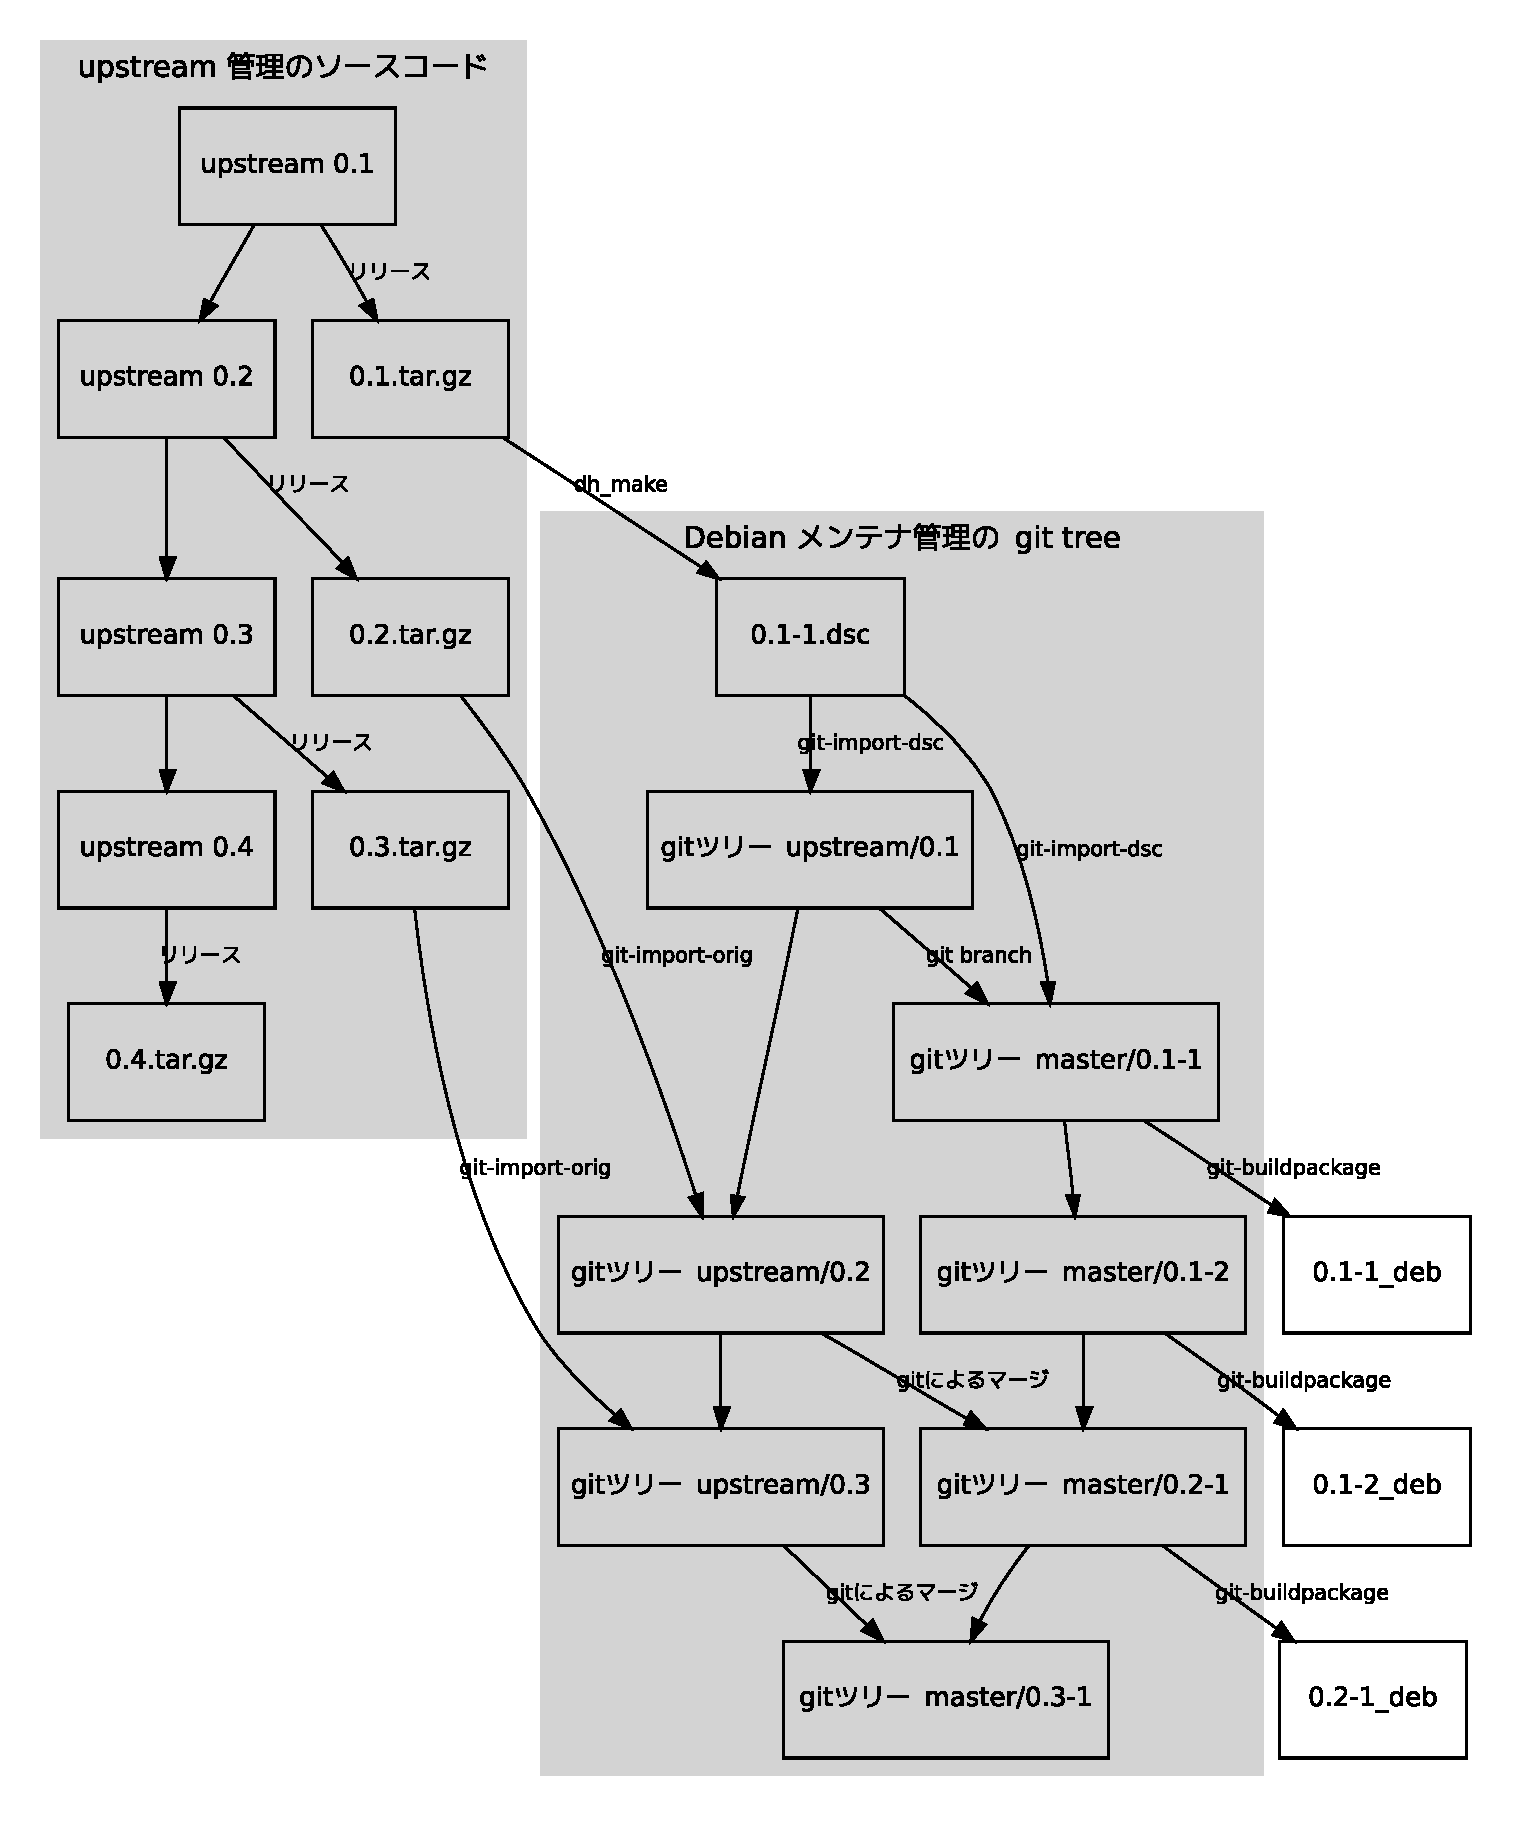
\includegraphics[height=1\vsize]{image200704/git-buildpackage.eps}
\end{frame}

\begin{frame}{git-buildpackage}
\begin{itemize}
 \item git-import-dsc
 \item git-import-orig
 \item git-buildpackage
\end{itemize}
\end{frame}

\begin{frame}{git-import-dsc}
 最初の Debian パッケージをインポートし、
 Debian ブランチとアップストリームのブランチを作成します
\end{frame}

\begin{frame}{git-import-orig}
 新しいアップストリームバージョンがリリースされた場合に
 アップストリームブランチにインポートし、
 Debian ブランチにマージします。
\end{frame}

\begin{frame}{git-buildpackage}
 git レポジトリからパッケージをビルドし、
 必要であればタグを付けます。
\end{frame}

\begin{frame}{}

利点: git-cherry / git-cherry-pick コマンドなどを利用して、まだマージされてい
 ない変更の一覧を確認できる

欠点: 一度コンフリクトがあるとその変更がマージのコミットとして記録される
 (quilt / dpatch との違い)

DebianのソースパッケージをみただけではSCMのレポジトリがどこにあるのかがわからな
 い。

\end{frame}

\begin{frame}{}
 
質問?

\end{frame}

\begin{frame}{Debian勉強会の今後の活動}
\begin{itemize}
 \item 5月:Debconf ネタ(superh, pbuilder-qemu)リハーサル? SCM の活用について? その他との連系について?
 \item 6月:スコットランドで開催
 \item 7月:
 \item 8月:
 \item 8月:
 \item 8月:
 \item 8月:
 \item 12月:反省会
\end{itemize}
 
\end{frame}

\end{document}
